\documentclass[a4paper, 12pt]{article}
\usepackage[utf8]{inputenc}
\usepackage[T1]{fontenc}
\usepackage[french]{babel}
\usepackage{lmodern}
\usepackage{graphicx, float, svg} 
\usepackage{amsmath, amssymb, amsthm}
\usepackage{listings}
\usepackage[listings,skins]{tcolorbox}
\usepackage{xcolor}

\usepackage[hyphens]{url}
\usepackage[pdfauthor = {{Prénom Nom}}, pdftitle = {{Titredocument}},pdfstartview = Fit, pdfpagelayout =
SinglePage, pdfnewwindow = true, bookmarksnumbered =
true, breaklinks, colorlinks, linkcolor = red, urlcolor =
black, citecolor = cyan, linktoc = all]{hyperref}

\usepackage[a4paper,margin=2.5cm]{geometry}

% \renewcommand{\familydefault}{\sfdefault}
\definecolor{codegreen}{rgb}{0,0.6,0}
\definecolor{codegray}{rgb}{0.5,0.5,0.5}
\definecolor{codepurple}{rgb}{0.58,0,0.82}
\definecolor{codeblue}{rgb}{0.0, 0.4, 0.8}
\definecolor{darkWhite}{rgb}{0.90,0.90,0.90}

\lstdefinestyle{bigCode}{
    backgroundcolor=\color{darkWhite},   
    commentstyle=\color{codegreen},
    keywordstyle=\color{codeblue},
    numberstyle=\tiny\color{codegray},
    stringstyle=\color{codepurple},
    basicstyle=\ttfamily\footnotesize,
    breakatwhitespace=false,         
    breaklines=true,                 
    captionpos=b,                    
    keepspaces=true,                 
    showspaces=false,                
    showstringspaces=false,
    showtabs=false,                  
    tabsize=2,
    language=c,
    morekeywords={free,malloc,nullptr,calloc,memcpy,realloc,bool,size_t,true,false}
}

\hypersetup{
  colorlinks=true,       % Enables colored links
  linkcolor=gray,        % Color for internal links (e.g., \ref and \autoref)
  citecolor=gray,        % Color for citations
  filecolor=gray,        % Color for file links
  urlcolor=gray          % Color for external URLs
}


\lstset{style=bigCode}

\NewTotalTCBox{\commandbox}{ s v }
{verbatim,colupper=black,colback=darkWhite!75!white,colframe=white,left=0pt,boxsep=0px,right=0pt,top=2px,bottom=2px}
{\IfBooleanT{#1}{\textcolor{red}{\ttfamily\bfseries > }}%
\lstinline[language=c,morekeywords={free,malloc,nullptr,calloc,memcpy,realloc,bool,size_t,true,false},keywordstyle=\color{codeblue}\bfseries]^#2^}

\newcommand{\code}{\commandbox}

\title{Distance de Jaccard}
\author{Maysaloon BILAL \& Tristan GROULT}
\date{\today}

\begin{document}

\begin{figure}[t]
    \centering
    \begin{minipage}{0.3\textwidth}
        \centering
        
\includegraphics[width=1\textwidth]{logo_univ.png}
    \end{minipage}
    \hfill
    \begin{minipage}{0.3\textwidth}
        \centering
        
\includegraphics[width=1\textwidth]{ufr_logo.png}
    \end{minipage}
\end{figure}

\maketitle

\clearpage\setcounter{page}{2}

{
\hypersetup{hidelinks} % Sommaire en "noir"
\renewcommand{\contentsname}{Sommaire}
\tableofcontents % Affichage du sommaire
}

\clearpage

\section{Introduction}


Ce projet consiste à développer un programme en langage C permettant de calculer la distance de Jaccard entre plusieurs fichiers texte, afin d’analyser leur similarité lexicale. La distance de Jaccard est une valeur comprise entre 0 et 1 : plus elle est proche de 0, plus les fichiers sont différents, et plus elle est proche de 1, plus ils sont similaires.

La distance de Jaccard entre deux ensembles $A$ et $B$ est définie par la formule :
$$
\text{Distance de Jaccard}(A, B) = 1 - \frac{|A \cap B|}{|A \cup B|}
$$

Le programme propose plusieurs modes d'affichage ainsi que des calculs personnalisés.  
Il est possible de mesurer la similarité entre les fichiers à l’aide de l’indice de Jaccard, que nous désignerons par la suite par \textit{Calcul de Jaccard}.  
Il est également possible d’afficher un graphe représentant l’appartenance des mots à leur(s) fichier(s), que nous nommerons \textit{Graphe de Jaccard}.  
Nous utiliserons le terme \textit{Calcul de Jaccard} pour faire référence à la réalisation ou la préparation de ces deux opérations.

Pour gérer efficacement les mots extraits des fichiers, nous avons utilisé une table de hachage. Sa gestion — ajout, suppression, affichage du graphe, etc. — est implémentée dans le module \code{jaccard}. Ce projet s’appuie également sur deux autres modules : le module \code{word} \autoref{word}, dédié à la création et la manipulation des mots, et le module \code{opt} \autoref{opt}, responsable du traitement des options en ligne de commande.

L’ensemble de ces composants est intégré et testé dans le fichier principal \code{main.c}, qui constitue le point d’entrée du programme.


\section{Conception et implémentation}

Dans cette section, nous expliquons les différentes étapes et approches utilisées pour implémenter le programme. Nous détaillerons la conception des modules, la gestion des fichiers et l’utilisation de la table de hachage.

\subsection{Module word}

\label{word}

Le module \code{word} a pour objectif de construire dynamiquement un mot caractère par caractère, afin de faciliter son traitement sans avoir à connaître sa taille à l’avance. Ce module est utilisé lors de la lecture des fichiers afin d'extraire chaque mot individuellement.

\subsubsection{Spécification}

Pour cela, nous utilisons une structure de données définie dans la \autoref{fig:word_schema}. Cette structure permet de stocker un mot, d'en gérer dynamiquement la taille, et de le manipuler facilement sans risque de dépassement mémoire. 

\begin{figure}[H]
\centering
\begin{tcolorbox}[enhanced,
colback=white,
colframe=codeblue,
fonttitle=\bfseries,
title=Schéma,
boxrule=2pt,
width=0.8\textwidth]
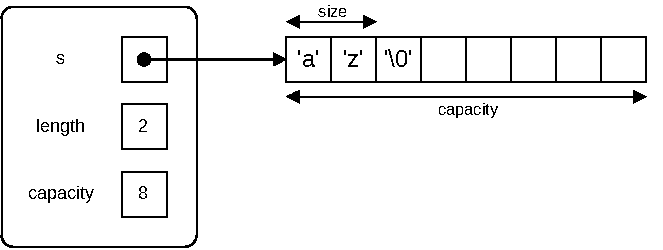
\includegraphics[width=\textwidth]{word_schema.pdf}
\end{tcolorbox}
\caption{Schéma de la structure word}
\label{fig:word_schema}
\end{figure}

\subsubsection{Implantation}

Lors de l’implémentation, nous avons défini une structure \code{struct word} (\autoref{fig:structure_word}) pour représenter dynamiquement un mot. Elle est composée de trois champs :

\begin{itemize}
\item Un champ \code{s} de type \code{char *} qui pointe vers un tableau de caractères contenant le mot.
\item Un champ \code{length} de type \code{size_t} qui représente la longueur actuelle du mot.
\item Un champ \code{capacity} de type \code{size_t} qui correspond à la taille totale allouée pour le mot.
\end{itemize}

Nous avons choisi une approche avec allocation mémoire dynamique, ce qui permet de s’adapter à la longueur des mots rencontrés, en multipliant par la constante \code{CAPACITY_MUL} la capacité du mot lorsque celle ci est atteinte.

\begin{figure}[h]
\centering
\begin{tcolorbox}[center upper,
enhanced,
colback=darkWhite,
boxrule=0pt,
frame hidden,
width=0.4\textwidth]
\begin{lstlisting}[style=bigCode]
struct word {
    char *s;
    size_t length;
    size_t capacity;
};
\end{lstlisting}
\end{tcolorbox}
\caption{Structure word}
\label{fig:structure_word}
\end{figure}

Nous avons développé plusieurs fonctions pour interagir avec ce module :

\begin{itemize}
\item \code{word_init()} : Initialise un mot vide en allouant une capacité minimale définie par la constante \code{CAPACITY_MIN}, et met la longueur à zéro.

\item \code{word_add()} : Ajoute un caractère à la fin du mot. Si la capacité est atteinte, elle est doublée avec \code{realloc()} pour permettre l'ajout de nouveaux caractères.

\item \code{word_reinit()} : Réinitialise le mot en mettant sa longueur à zéro, ce qui permet de le réutiliser sans réallouer de mémoire.

\item \code{word_get()} : Renvoie un pointeur vers la chaîne de caractères actuelle.

\item \code{word_get_clean()} : Copie le contenu réel du mot dans une destination passée en paramètre, sans les éventuels caractères résiduels.

\end{itemize}



\subsection{Module opt}
\label{opt}

Le module \code{opt} a pour objectif de gérer les options de la ligne de commande, en les analysant puis en les restituant sous une forme exploitable par le reste du programme.
Dans le cadre de ce projet, les options suivantes sont nécessaires :

\begin{itemize}
\item \code{-g} : Affiche le graphe de Jaccard.
\item \code{-p} : Ignore les caractères de ponctuation lors de l'analyse.
\item \code{-iVALUE} : Spécifie la longueur maximale des mots.
\item \code{-} : Utilise l'entrée standard comme source.
\item \code{--} : Indique que l'argument suivant est un nom de fichier.
\item \code{-u} : Affiche les informations d'utilisation de l'exécutable.
\item \code{-v} : Affiche la version de l'exécutable.
\item \code{-?} : Affiche l’aide de l’exécutable.
\end{itemize}

\subsubsection{Spécification}

Pour représenter les options analysées, nous utilisons une structure de données illustrée dans la \autoref{fig:opt_schema}.
Nous avons choisi de limiter le nombre de fichiers grâce à une constante nommée \code{MAX_FILES}. Ce choix permet d’assurer une consommation mémoire bornée et facilite l'intégration avec les contraintes d’implémentation du module \code{jaccard}.

\begin{figure}[H]
\centering
\begin{tcolorbox}[enhanced,
colback=white,
colframe=codeblue,
fonttitle=\bfseries,
title=Schéma,
boxrule=2pt,
width=0.8\textwidth]
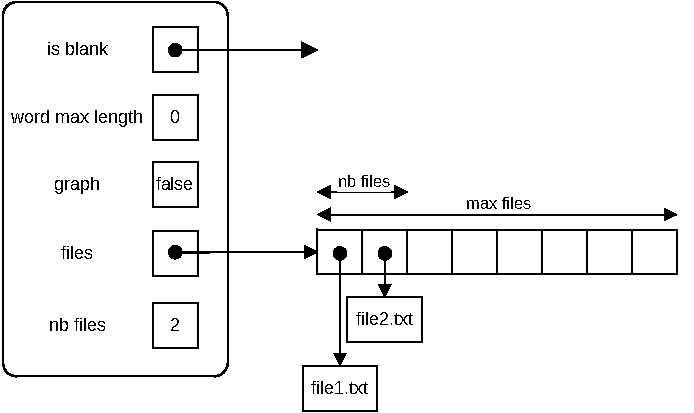
\includegraphics[width=\textwidth]{opt_schema.pdf}
\end{tcolorbox}
\caption{Schéma de la structure opt}
\label{fig:opt_schema}
\end{figure}

\subsubsection{Implémentation}

L’implémentation repose sur l’utilisation d’une structure \code{struct opt}, définie comme suit (\autoref{fig:structure_opt}) :

\begin{itemize}
\item \code{isBlank} : Pointeur vers une fonction \code{int(int)} déterminant les caractères séparateurs de mots.
\item \code{word_max_length} : Entier définissant la longueur maximale d’un mot (0 signifie aucune limite ; valeur par défaut : 0).
\item \code{graph} : Booléen indiquant si le graphe de Jaccard doit être affiché.
\item \code{files} : Tableau de chaînes de caractères représentant les noms des fichiers à analyser.
\item \code{nb_files} : Nombre de fichiers fournis en argument.
\end{itemize}

\begin{figure}[h]
\centering
\begin{tcolorbox}[center upper,
enhanced,
colback=darkWhite,
boxrule=0pt,
frame hidden,
width=0.5\textwidth]
\begin{lstlisting}[style=bigCode]
struct opt {
    int (*isBlank)(int);
    int word_max_length;
    bool graph;
    char const **files;
    int nb_files;
};
\end{lstlisting}
\end{tcolorbox}
\caption{Structure opt}
\label{fig:structure_opt}
\end{figure}

Afin de permettre une gestion homogène de l’entrée standard, nous la représentons sous la forme d’une chaîne vide (\code{""}), en la définissant via une macro \code{STDIN}. Cette chaîne est utilisée comme nom de fichier, en tirant parti du fait qu’aucun système courant ne l’autorise comme nom valide.

Seules les options courtes ont été implémentées, comme listé plus haut. Pour l’option \code{-iVALUE}, la valeur doit être directement collée à l’option (par exemple \code{-i3}), l’espacement (\code{-i 3}) n’étant pas pris en charge.

Enfin, toutes les options sont définies via des macros constantes. Le préfixe des options courtes est également paramétrable, ce qui rend l’ensemble du module facilement adaptable à d’autres conventions si nécessaire.


\subsection{Module Jaccard}

Le module \code{jaccard} a pour objectif de réaliser le calcule de Jaccard en donnant la possibilité d'ajouter des mots au calcule ainsi que de gérer l'affichage du graphe ou le calcule de la distance.

\subsubsection{Spécification}

Pour réaliser cella, nous utilisons une structure de données définie dans la \autoref{fig:jaccard_shema}. Cette structure permet de sauvgarder les éléments utilisé pour réaliser le calcule de la distance ansi que les autres strucure donné que nous avons décidé d'utiliser. 

\begin{figure}[H]
    \centering
    \begin{tcolorbox}[enhanced,
    colback=white,
    colframe=codeblue,
    fonttitle=\bfseries,
    title=Schéma,
    boxrule=2pt,
    width=0.8\textwidth]
    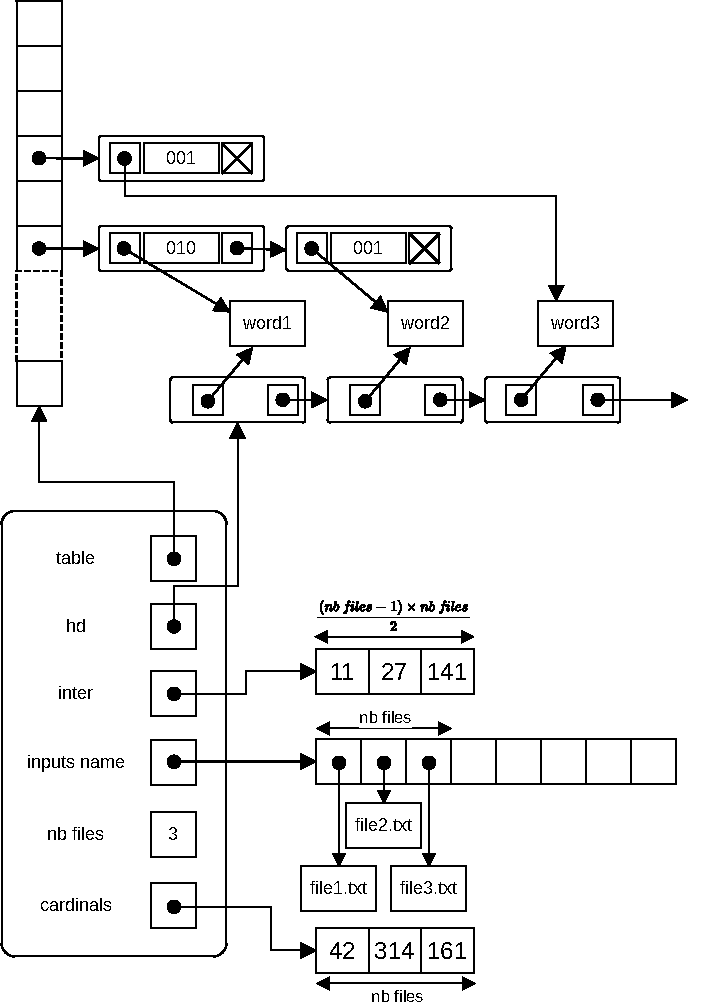
\includegraphics[width=\textwidth]{jaccard_schema.pdf}
    \end{tcolorbox}
    \caption{Schéma de la structure jaccard}
    \label{fig:jaccard_shema}
    \end{figure}
\end{document}